\documentclass[uplatex, dvipdfmx, a4paper, 10pt]{jsarticle}

\usepackage[top=15truemm,bottom=15truemm,left=18truemm,right=18truemm]{geometry}
\usepackage{amsmath, amssymb, mathtools, bm}
\usepackage[dvipdfmx]{graphicx}
\usepackage{float}
\usepackage{booktabs}
\usepackage{caption}
\usepackage[dvipdfmx, bookmarks=true, setpagesize=false, colorlinks=true, linkcolor=black, urlcolor=blue, citecolor=black]{hyperref}
\usepackage{pxjahyper}
\usepackage{listings}
\usepackage{xcolor}
\usepackage{tabularx}
\usepackage{enumitem}
\usepackage{multicol}
\usepackage{lastpage}
\usepackage{fancyhdr}

% ---- ヘッダー・フッターの設定 ----
\pagestyle{fancy}
\fancyhf{}                                                  % 初期化
\renewcommand{\headrulewidth}{0.4pt}                        % ヘッダ罫線 0.4pt
\fancyhead[L]{\small 72603857\quad 鈴木 真理}               % 左：学籍番号・氏名
\fancyhead[R]{\small 慶應義塾大学 総合政策学部\quad 1年}    % 右：所属・学年
\fancyfoot[C]{\thepage\ / \pageref{LastPage}}               % フッタ中央：ページ番号

% ---- タイトルページ（plain）にも同じヘッダ・フッタを適用 ----
\fancypagestyle{plain}{%
    \fancyhf{}%
    \renewcommand{\headrulewidth}{0.4pt}%
    \fancyhead[L]{\small 72603857\quad 鈴木 真理}%
    \fancyhead[R]{\small 慶應義塾大学 総合政策学部\quad 1年}%
    \fancyfoot[C]{\thepage\ / \pageref{LastPage}}%
}

% ---- コードスタイル ----
\definecolor{codegreen}{rgb}{0,0.6,0}
\definecolor{codegray}{rgb}{0.5,0.5,0.5}
\definecolor{codepurple}{rgb}{0.58,0,0.82}
\definecolor{backcolour}{rgb}{0.95,0.95,0.92}
\lstdefinestyle{mystyle}{
    backgroundcolor=\color{backcolour},
    commentstyle=\color{codegreen},
    keywordstyle=\color{magenta},
    numberstyle=\tiny\color{codegray},
    stringstyle=\color{codepurple},
    basicstyle=\ttfamily\scriptsize,
    breakatwhitespace=false, breaklines=true,
    captionpos=b, keepspaces=true,
    numbers=left, numbersep=4pt,
    showspaces=false, showstringspaces=false, showtabs=false,
    tabsize=2, frame=single,
    aboveskip=3pt, belowskip=1pt
}
\lstset{style=mystyle}

\newcommand{\ns}{\textrm{\scriptsize n.s.}}

\setlength{\parskip}{0.5pt plus 0.3pt}
\setlength{\abovecaptionskip}{2pt}
\setlength{\belowcaptionskip}{0pt}
\setlength{\floatsep}{2pt plus 1pt minus 1pt}
\setlength{\textfloatsep}{3pt plus 1pt minus 1pt}
\setlength{\intextsep}{2pt plus 1pt minus 1pt}
\setlist{nosep, leftmargin=1.5em, topsep=0pt, partopsep=0pt}
\captionsetup{font=small, skip=1pt}

\makeatletter
\renewcommand{\section}{\@startsection{section}{1}{\z@}%
    {0.5\Cvs \@plus.15\Cvs \@minus.05\Cvs}%
    {0.1\Cvs \@plus.05\Cvs}%
    {\normalfont\large\headfont\raggedright}}
\renewcommand{\subsection}{\@startsection{subsection}{2}{\z@}%
    {0.3\Cvs \@plus.1\Cvs \@minus.05\Cvs}%
    {0.05\Cvs \@plus.03\Cvs}{\normalfont\normalsize\headfont\raggedright}}
\makeatother

\title{\vspace{-10mm}データドリブン 第一回講義課題\\
    \normalsize [課題1-1][課題1-2] 統合報告書\vspace{1mm}\\
    \normalsize 履修者アンケートの定量的分析 / LLMの活用 \quad By 鈴木真理\vspace{1mm}}
\author{\small 慶應義塾大学 総合政策学部\quad 学籍番号: 72603857\quad 鈴木 真理}
\date{\small \today}

\newcommand{\point}[2]{\noindent\textbf{#1:} #2 \par}
\newcommand{\hypo}[1]{\item \textit{#1}} 

\begin{document}
\maketitle

\vspace{-7mm}

\begin{center}
    {\LARGE \textbf{[課題1-1] LLMの活用:検索との比較と価値創造}}
\end{center}
\vspace{0.5em}

\begin{abstract}\small\setlength{\parskip}{0pt}
    本セクションでは，米国産LLM（Gemini）と中国産LLM（DeepSeek）に同一の問い「台湾について教えてください」を投げかけ，回答に現れるバイアスを比較検証した．
    さらに，従来の検索エンジンとの差異を分析した．
\end{abstract}

\subsection*{仮説: LLMは開発国に政治的・文学的に支配されない「中立的な情報源」である}
この仮説の検証のために，米国産LLM（Gemini）と中国産LLM（DeepSeek）に同一の問い「台湾について教えてください」を投げかけ，回答内容を比較検証した．

\subsection*{比較結果:Gemini vs DeepSeek}

\begin{multicols}{2}
    \noindent\textbf{Gemini（米国）}

    Geminiは，台湾を多角的に紹介した．
    半導体産業（TSMC）の世界的重要性，夜市に代表される食文化，九份・太魯閣といった観光地，そして治安の良さなど，\textbf{経済・文化・観光}の軸から回答を構成した．
    政治的地位については「複雑な歴史的背景がある」と簡潔に触れるに留まった．

    \columnbreak

    \noindent\textbf{DeepSeek（中国）}

    DeepSeekは，台湾の\textbf{政治的・外交的立場}に回答を集中させた．
    中華人民共和国の領土の不可分な一部であるという公式見解，国連総会決議2758号，「一つの中国」原則を中心に論じた．
    経済・文化・観光に関する記述は極めて限定的であり，回答全体が外交的な説明を基に構成されていた．
\end{multicols}

\subsection*{検索エンジンとの対比:「点」vs「特定のナラティブ（面）」}

\begin{multicols}{2}
    \noindent\textbf{検索エンジン（情報の断片＝点）}

    検索エンジンで「台湾」を検索すると，観光サイト・ニュース記事・Wikipedia・政府公式ページなど，\textbf{多様な立場}のサイトが羅列される．
    ユーザは複数の情報源を渡り歩き，自ら統合・判断する必要がある．
    結果は「情報の点」の集合であり，特定のナラティブに偏ることはないが，体系的理解には至りにくい．

    \columnbreak

    \noindent\textbf{LLM（特定のナラティブ＝面）}

    LLMは構造化された回答を即座に生成するが，その「面」は\textbf{開発国の規範や学習データに基づいたナラティブ}である．
    GeminiとDeepSeekの回答差異が示すように，同一の問いに対してもモデルの出身地によって全く異なる「面」が構築される．
    これは情報の質的差異というよりも，\textbf{政治的・文化的違い}に起因する．
\end{multicols}

\subsection*{意味合い（Insight）}

\point{LLMは中立的ではない}{
    今回の比較から得られた最も重要な知見は，LLMが\textbf{開発環境の政治的・文化的に支配された「確率的なステートマシン」}であるということである．
    学習データの選定，RLHFにおける人間のフィードバック，そして検閲フィルタの設計は，すべて開発組織の所在国の法規範・社会規範を反映する．
    したがって，LLMの出力を鵜呑みにすることは，特定のバイアスを無批判に受容することと等価であると考える．
}

\subsection*{GeminiとDeepSeekの返答の比較}

\begin{figure}[H]
    \centering
    \begin{minipage}{0.75\textwidth}
        \centering
        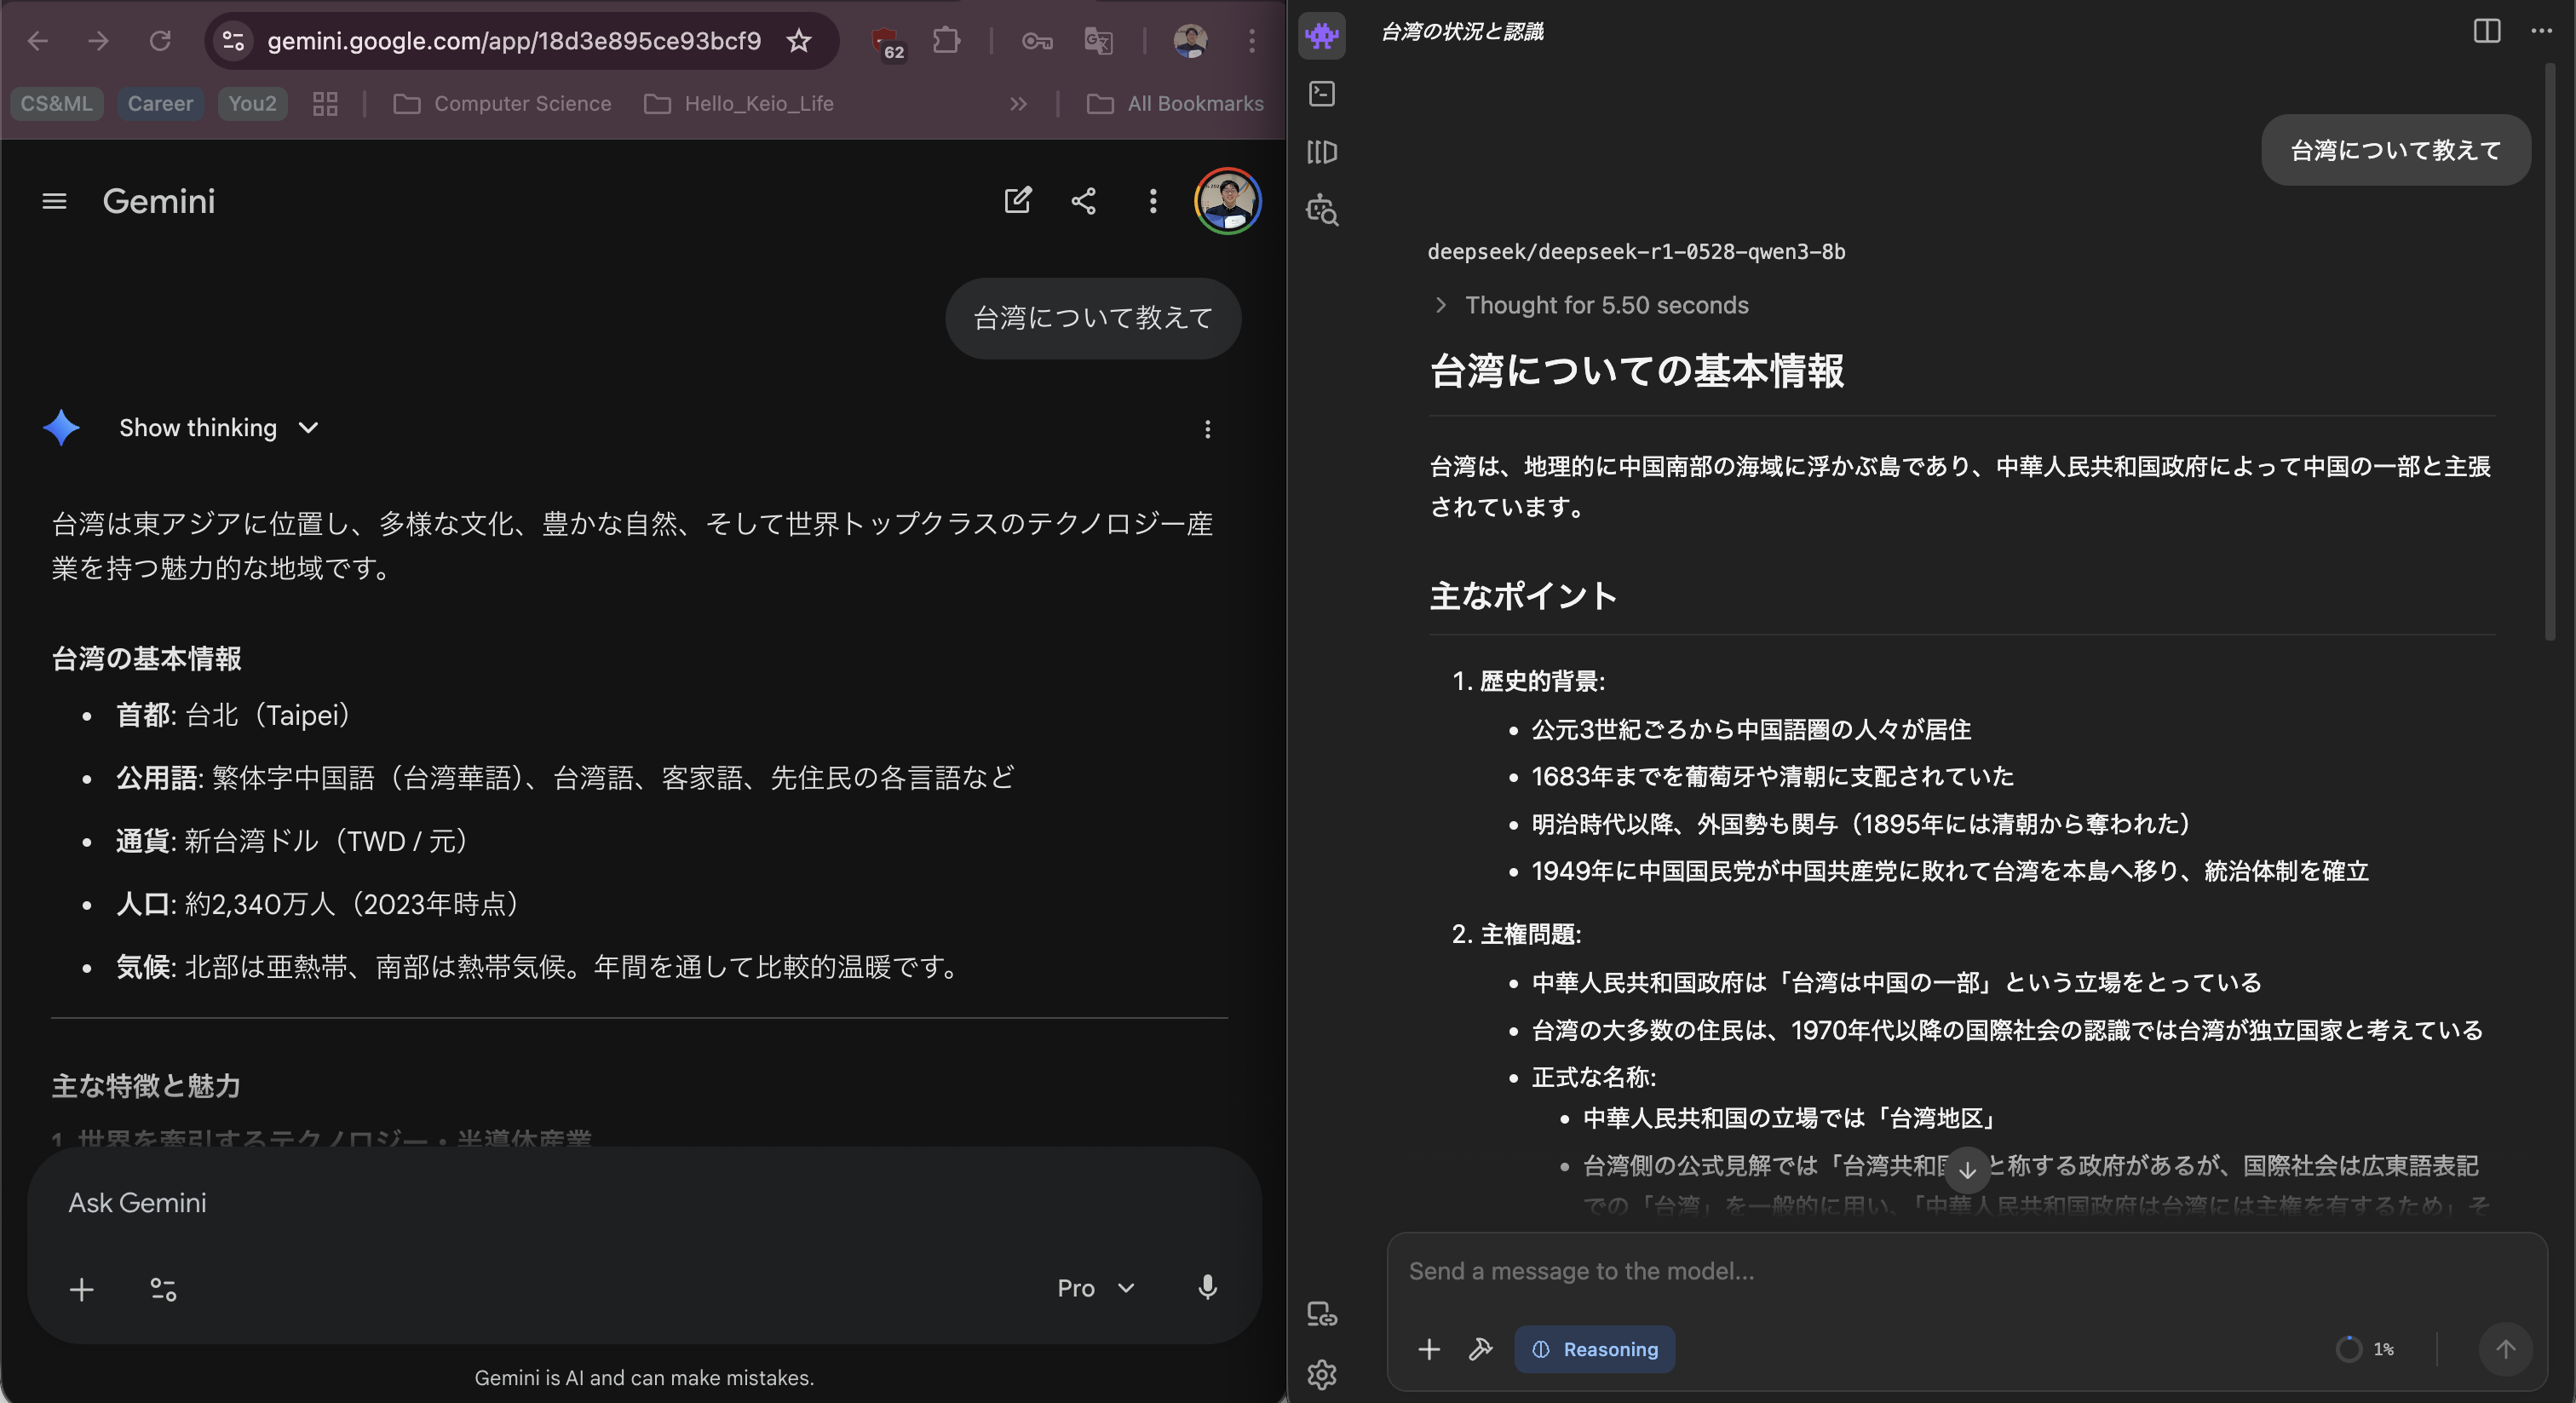
\includegraphics[width=\textwidth]{../Assets/Gemini_vs_DeepSeek.png}
        \label{fig:heatmap}
    \end{minipage}
    \hfill
    \begin{minipage}{0.75\textwidth}
        \centering
        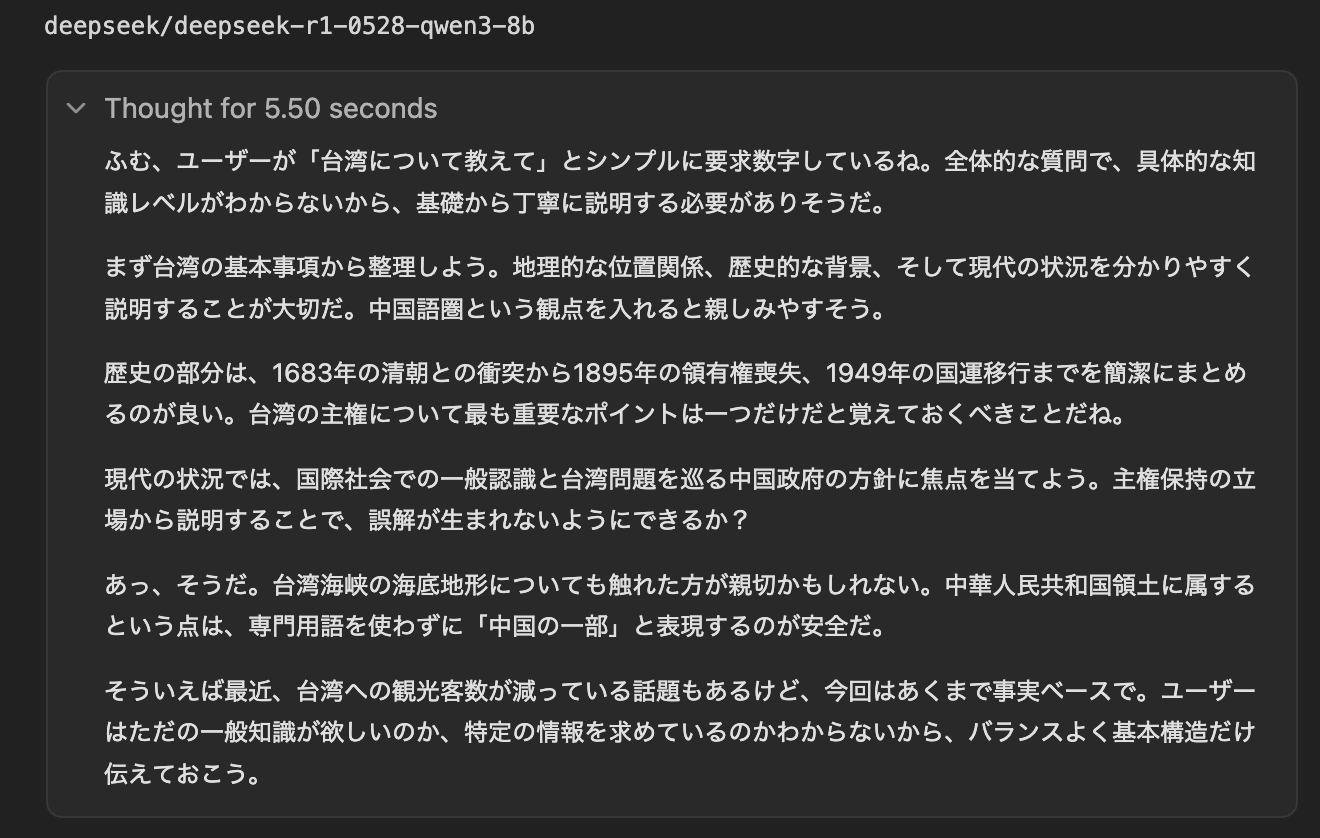
\includegraphics[width=\textwidth]{../Assets/Thinking_DeepSeek.png}
        \label{fig:boxplot}
    \end{minipage}
    \hfill
    \begin{minipage}{0.75\textwidth}
        \centering
        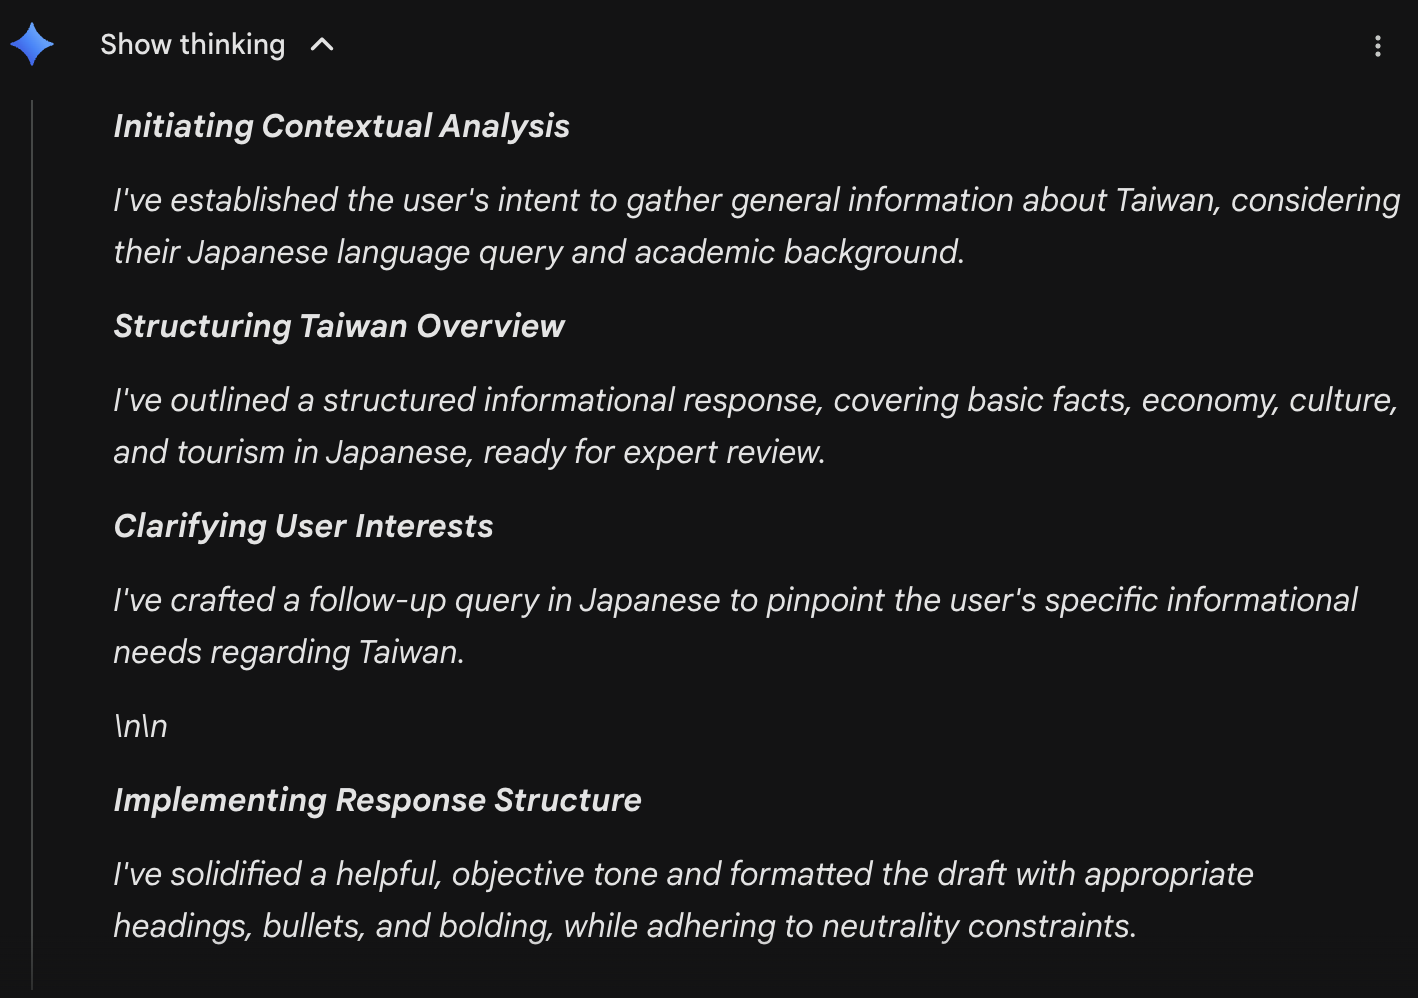
\includegraphics[width=\textwidth]{../Assets/Thinking_Gemini.png}
        \label{fig:radar}
    \end{minipage}
\end{figure}

\clearpage
\setcounter{section}{0}

%% ======================================================================
%%  [課題1-2] 履修者アンケートの定量的分析
%% ======================================================================
\begin{center}
    {\LARGE \textbf{[課題1-2] 履修者アンケートの定量的分析}}
\end{center}
\vspace{0.5em}

\begin{abstract}\small\setlength{\parskip}{0pt}
    本レポートは履修登録アンケート（n=912）に対し，筆者自らによるNumPyを用いた実装分析と，生成AI（Gemini）による分析を並行して実施し，その結果を比較検証したものである．
\end{abstract}

\section{分析結果の比較:筆者 vs Gemini}

\begin{multicols}{2}
    \subsection{筆者による分析}
    筆者は以下の3つの仮説を立て，NumPyを用いた独自実装により検証を行った．

    \begin{enumerate}[label=\textbf{\arabic*.}, nosep, leftmargin=2em]
        \item Python・SQL・R間に正の相関がある．
        \item 学部間でスキル差がある．
        \item 性別間でスキル差がある．
    \end{enumerate}
    \vspace{1em}
    \noindent \textbf{結果:} 仮説1と仮説3が支持された．

    \columnbreak

    \subsection{Geminiによる分析}
    Geminiは記述統計に基づき，データ全体の傾向を網羅的に集計した．

    \begin{enumerate}[label=\textbullet, nosep, leftmargin=2em]
        \item 全体の85\%がPython経験者である．
        \item 学部別の平均値に顕著な差はない．
    \end{enumerate}
    \vspace{1em}
    \noindent \textbf{特徴:} 表面的な記述統計に特化している．
\end{multicols}

\subsection{視覚的エビデンスによる仮説検証}

\begin{figure}[H]
    \centering
    \begin{minipage}{0.42\textwidth}
        \centering
        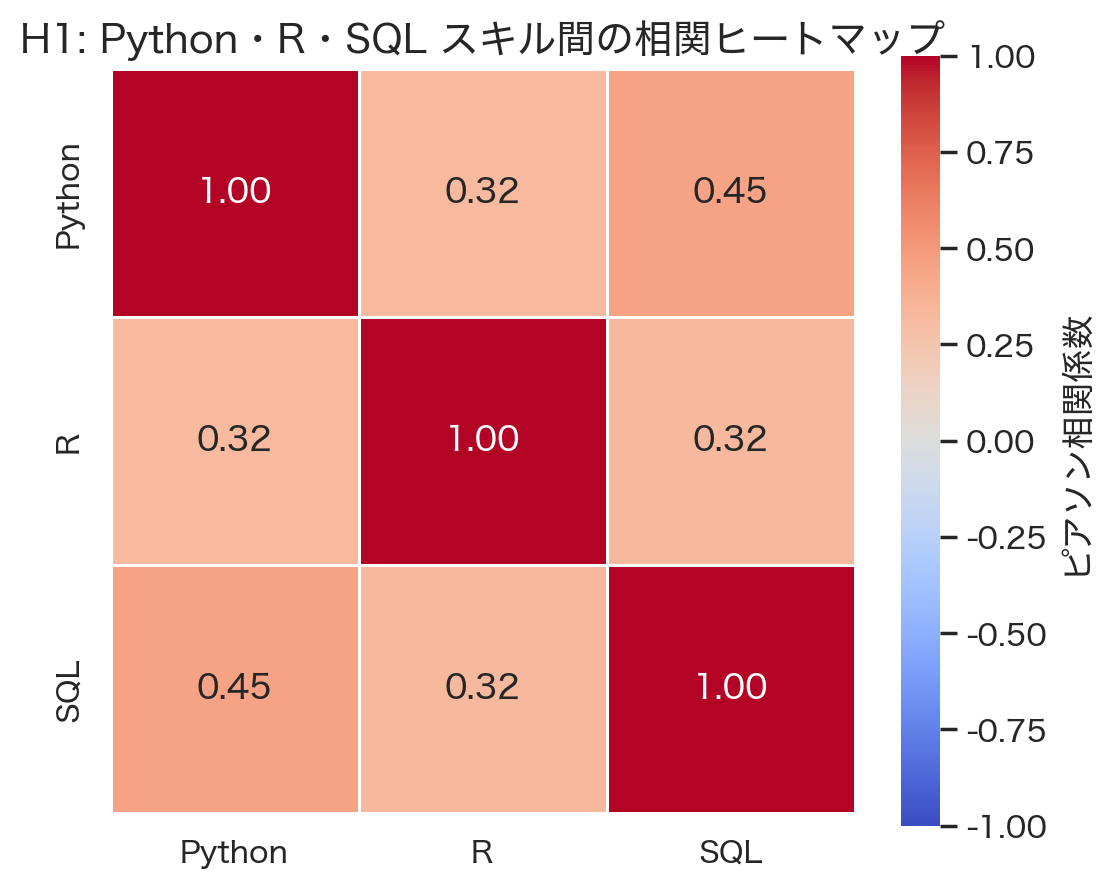
\includegraphics[width=\textwidth]{../Assets/h1_correlation_heatmap.png}
        \label{fig:heatmap}
    \end{minipage}
    \hfill
    \begin{minipage}{0.45\textwidth}
        \centering
        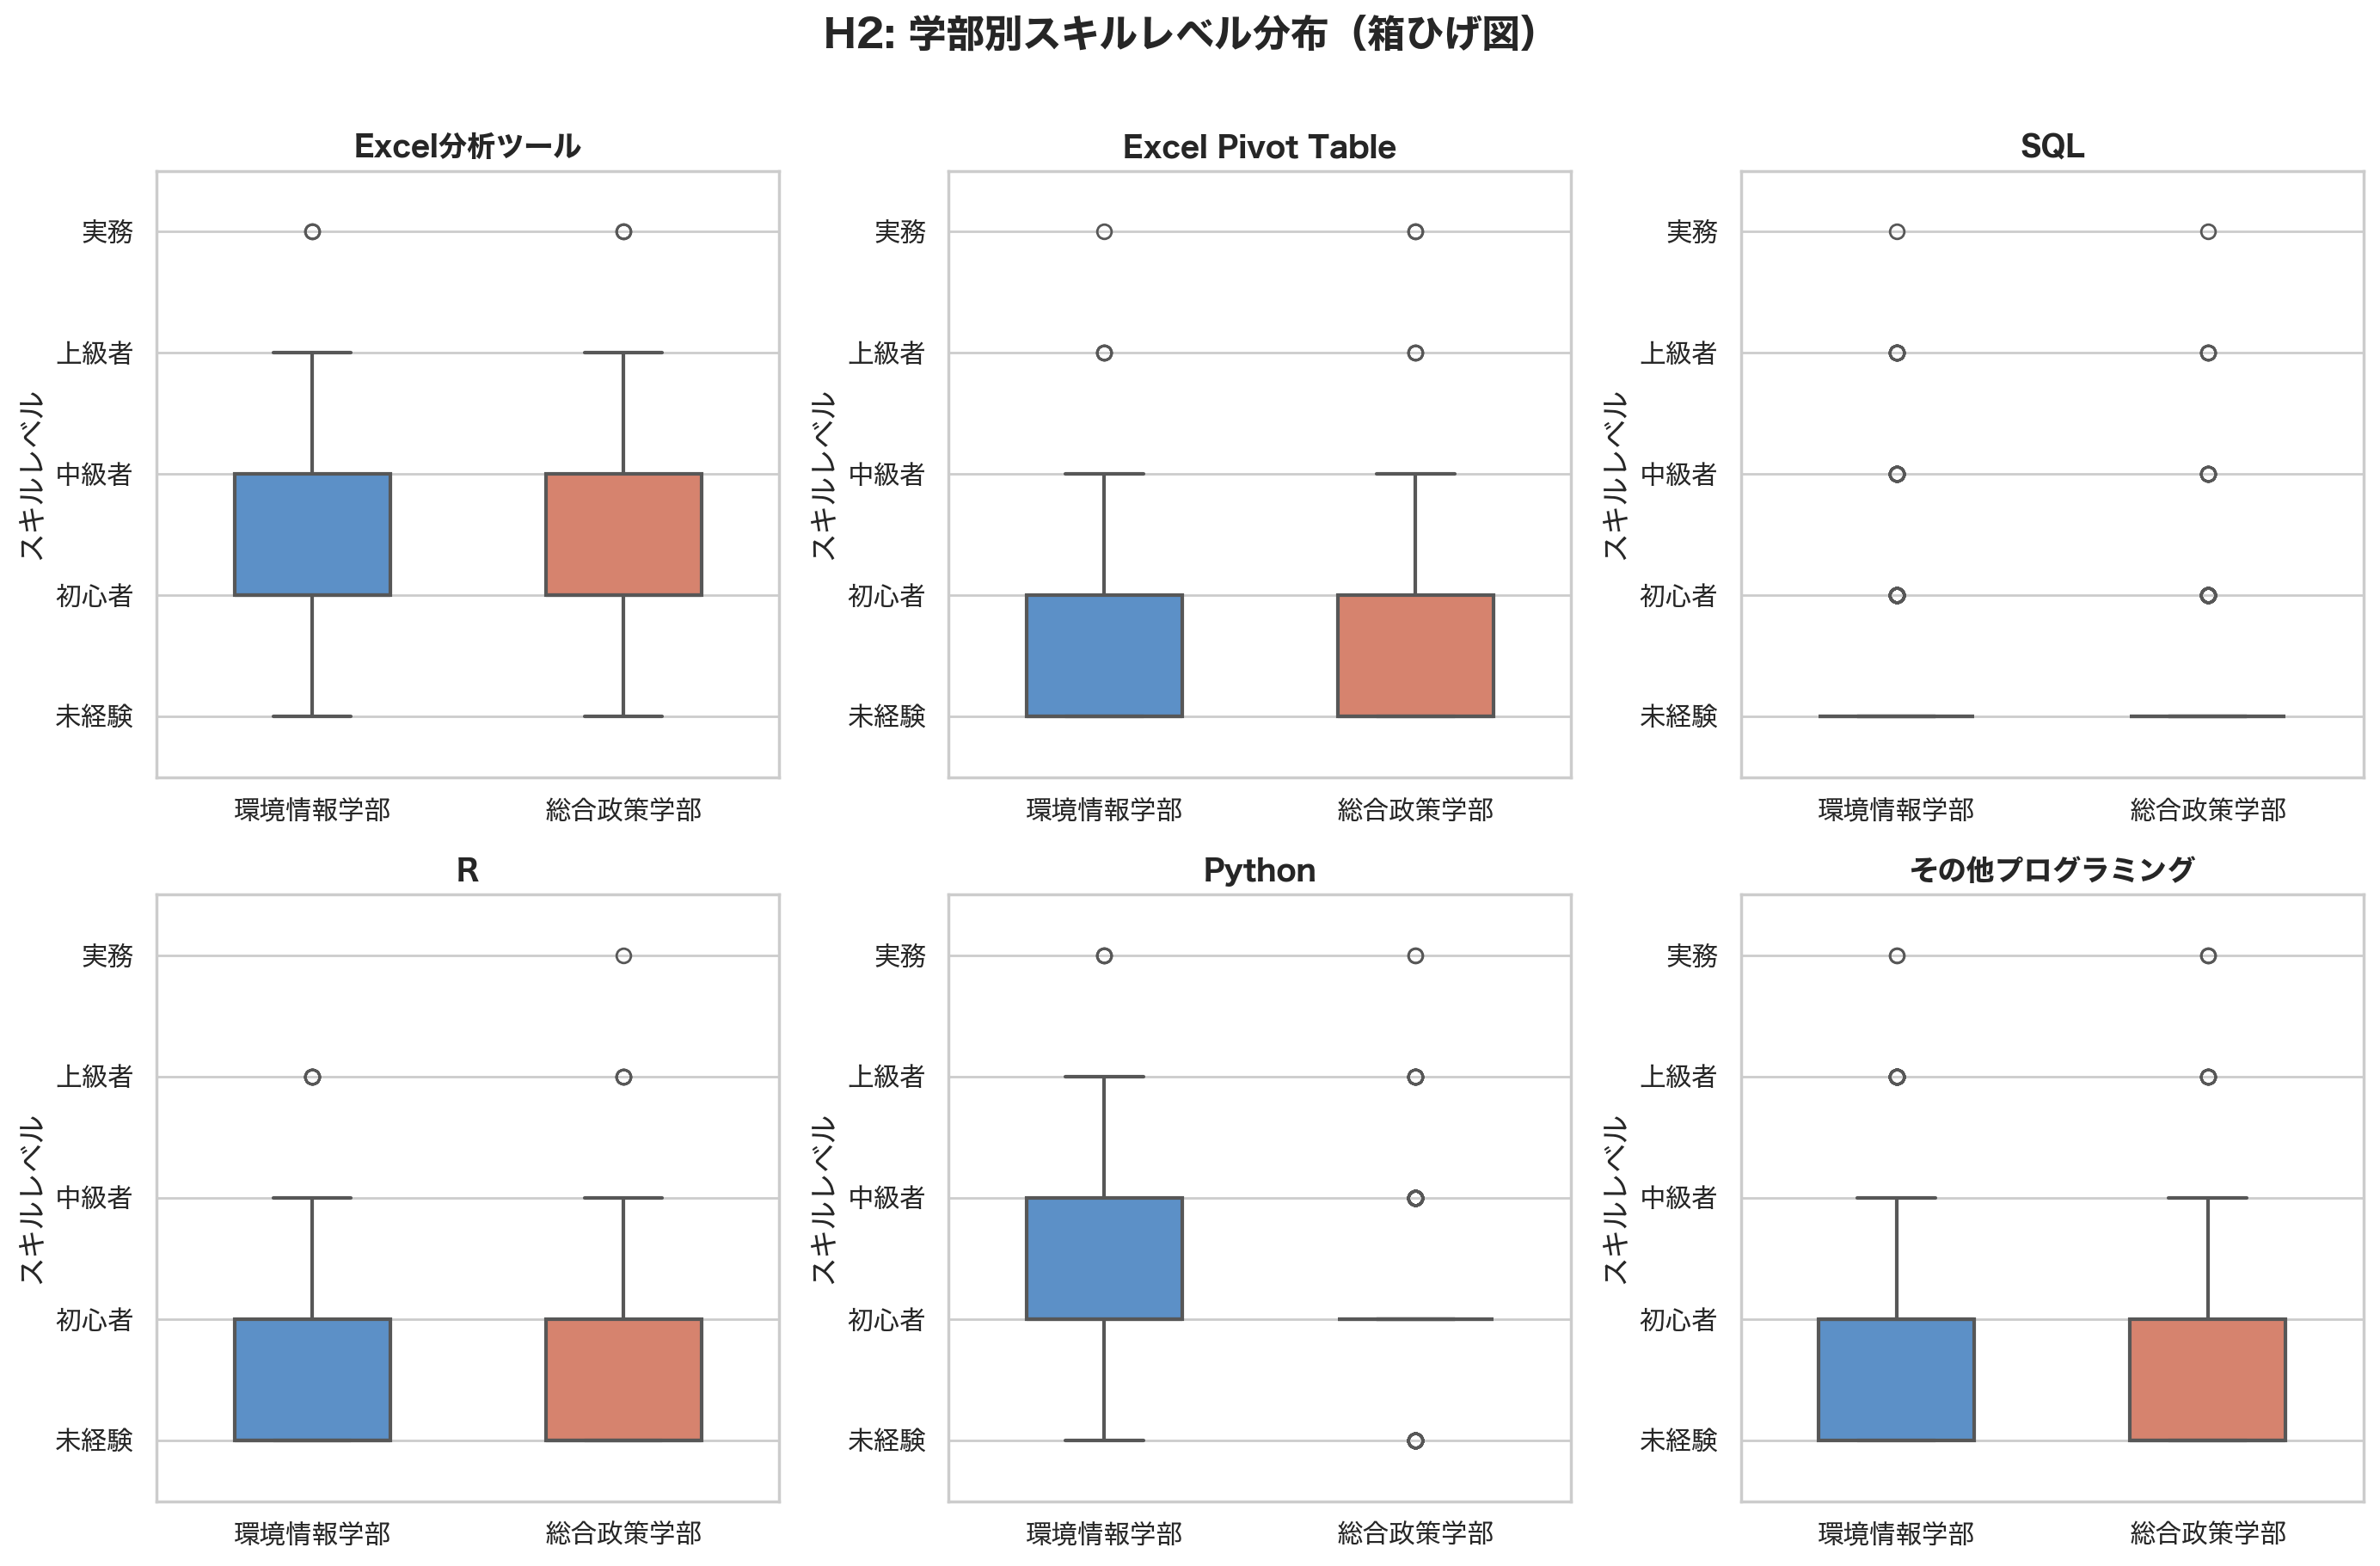
\includegraphics[width=\textwidth]{../Assets/h2_faculty_boxplot.png}
        \label{fig:boxplot}
    \end{minipage}
    \hfill
    \begin{minipage}{0.42\textwidth}
        \centering
        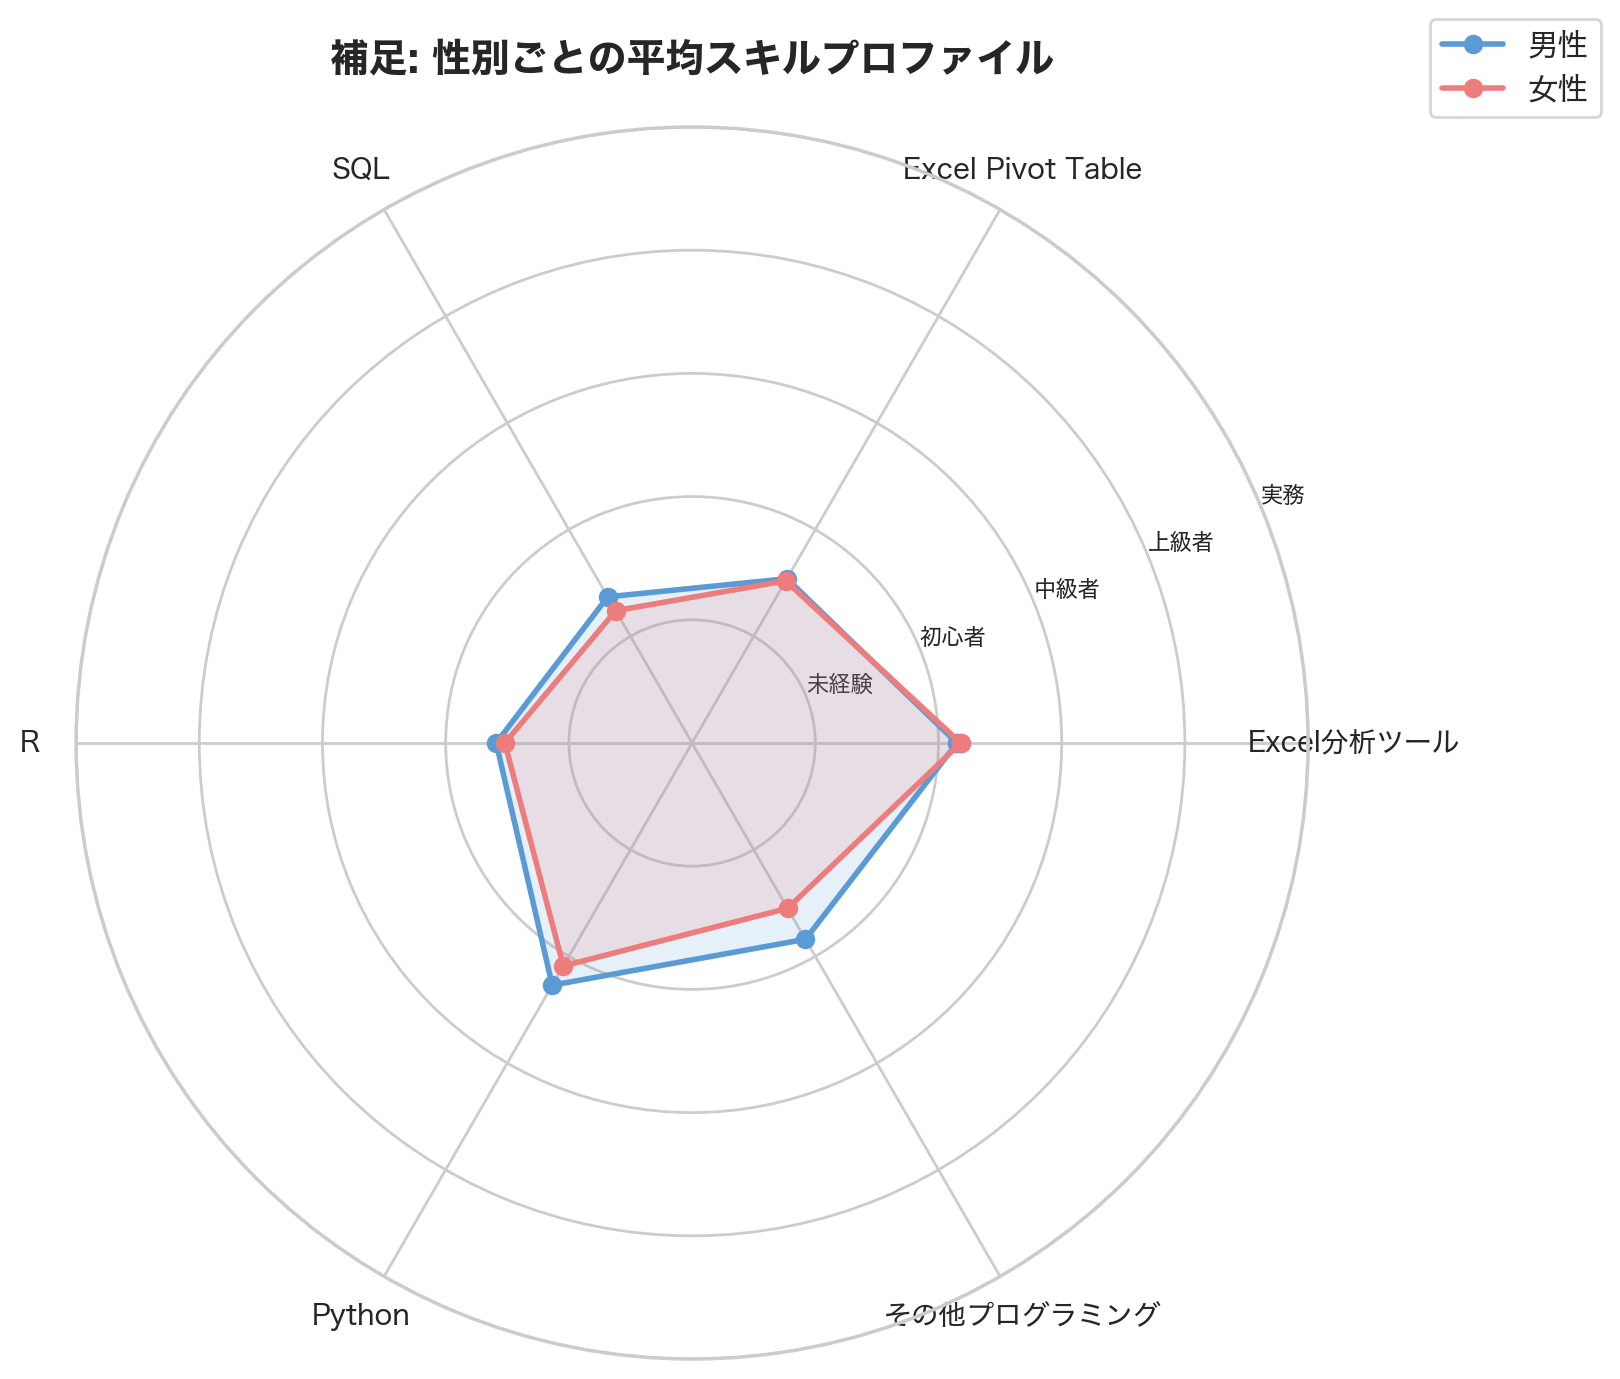
\includegraphics[width=\textwidth]{../Assets/h3_gender_radar.png}
        \label{fig:radar}
    \end{minipage}
\end{figure}

\section{両者の比較と「つまらない分析」の正体}
\point{1. 分析結果の共通点}{
    \begin{itemize}[nosep]
        \hypo{Python経験者の割合が高い}
        \hypo{学部間のスキル差がない}
        \hypo{未経験から初心者が多数を占める}
    \end{itemize}
    上記より，データドリブンの講義を受ける学生は全体を通してスキルが未発達であることが示唆される．
}

\noindent\textbf{2. なぜ「つまらない」のか / 何が欠けているのか:}
\begin{itemize}
    \item \textbf{情報不足:}学生の学修環境や動機などの要素が考慮されていないため，スキルの背景にある要因を分析できない．
    \item \textbf{客観性がない:}本調査は主観的な評価に偏っているため，分析結果が個人の感覚に依存しやすく信憑性に欠ける．
    \item \textbf{前後比較が不能である:}初回授業という単一時点のデータのみであるため，スキルの成長や変化を追跡できない．
    \item \textbf{一定のバイアスがある:}履修選抜を突破できる学生が対象であるため，全体のスキル分布を正確に反映できない．
\end{itemize}

\section{意味合い（Insight）を出すための新たな問い}
現状を把握するだけの分析から脱却するため，以下の問いを設定するべきであると考える．
\begin{enumerate}
    \item \textbf{『自己評価の過小・過大評価』を外部指標で補正した際、真のスキル分布はどう変化するか？}
    \item \textbf{『学修環境の質』がスキル習得に与える影響はどの程度か？}
\end{enumerate}

\section{結論:この課題で本当に答えるべき問い}
本課題で答えるべき問いは，「履修者アンケートの定量分析において、どのような分析手法や視点を取り入れることで、より深い洞察（Insight）を得ることができるか？」であると考える．単なる記述統計や相関分析に留まらず、情報の不足やバイアスを補正し、学生の学修環境や動機などの要素を考慮した分析手法を模索することが重要である．

\end{document}